\documentclass[12pt, a4paper]{article}
\usepackage[utf8]{inputenc}
\usepackage{geometry}
\geometry{top=3cm, bottom=3cm, left=3cm, right=3cm}
\usepackage{graphicx}
\usepackage{listings}
\usepackage{xcolor}
\usepackage{hyperref}
\usepackage{tikz}
\usetikzlibrary{shapes.geometric, arrows.meta, positioning}

% --- Konfigurasi Format Kode Rust ---
\definecolor{rustcomment}{rgb}{0.0, 0.5, 0.0}
\definecolor{rustkeyword}{rgb}{0.0, 0.0, 0.8}
\definecolor{ruststring}{rgb}{0.63, 0.125, 0.94}
\lstset{
    language=C++, 
    basicstyle=\ttfamily\footnotesize,
    keywordstyle=\color{rustkeyword}\bfseries,
    commentstyle=\color{rustcomment}\itshape,
    stringstyle=\color{ruststring},
    morekeywords={fn, let, mut, match, loop, impl, struct, f32, String, bool, println, new, self},
    numbers=left,
    numberstyle=\tiny\color{gray},
    stepnumber=1,
    breaklines=true,
    frame=single,
    tabsize=4,
    showstringspaces=false
}

\begin{document}

% ==================== 1. COVER ==================== %
\begin{titlepage}
    \centering
    \vspace*{1cm}
    
    {\Large \bfseries EVALUASI TENGAH SEMESTER (ETS) \par}
    {\Large \bfseries ALGORITMA DAN PEMROGRAMAN \par}
    \vspace{0.5cm}
    {\large \bfseries Semester Genap 2025/2026 \par}
    
    \vspace{2cm}
    
    {\Large \bfseries PROJECT BASED LEARNING (PBL) \par}
    {\Large \bfseries Pengembangan Sistem Instrumentasi Pengukuran dan Kontrol Berbasis Rust \par}
    \vspace{1cm}
    {\large \bfseries Studi Kasus: Sistem Monitoring Kelembaban dan Kualitas Udara \par}
    
    \vspace{3cm}
    
    \textbf{Disusun Oleh:} \par
    \vspace{0.5cm}
    Hageng Priyambada Alim \hspace{1cm} (NRP: 2042251089) \par 
    Aurepope Kasih Lamarebon \hspace{1cm} (NRP: 2042241122) \par
    
    \vspace{3cm}
    \textbf{Dosen Pengampu:} \par
    Ahmad Radhy, S.Si., M.Si. \par
    
    \vfill
    
    {\large \bfseries DEPARTEMEN TEKNIK INSTRUMENTASI \par}
    {\large \bfseries INSTITUT TEKNOLOGI SEPULUH NOPEMBER \par}
    {\large \bfseries SURABAYA \par}
    {\large \bfseries 2026 \par}
    
\end{titlepage}

\newpage
\tableofcontents
\newpage

% ==================== 2. PENDAHULUAN ==================== %
\section{Pendahuluan}
Sistem pemantauan kualitas udara dan kondisi lingkungan kini menjadi kebutuhan krusial dalam perlindungan kesehatan publik dan lingkungan. Penggunaan teknologi \textit{Internet of Things} (IoT) memungkinkan perolehan informasi kualitas udara secara \textit{real-time} dan akurat.

Proyek ETS ini bertujuan mengembangkan purwarupa perangkat lunak berbasis Rust untuk memantau kelembaban dan konsentrasi gas polutan. Rust dipilih karena keunggulannya dalam keamanan memori, yang sangat penting untuk aplikasi instrumentasi yang berjalan terus-menerus.

\subsection{Kajian Pustaka dan Sitasi}
Sistem ini dirancang dengan merujuk pada integrasi berbagai sensor seperti DHT11 untuk suhu dan kelembaban, serta MQ135 untuk menganalisis kadar gas di lingkungan. Sebagaimana dijelaskan oleh Garg dkk. (2025), sensor DHT11 mendeteksi suhu dan kelembaban melalui \textit{output} digital yang dihubungkan langsung ke mikrokontroler seperti ESP32.

Selain aspek pembacaan, sistem keamanan otomatis menjadi komponen vital. Chanthakit dan Rattanapoka (2018) menekankan bahwa ketika nilai data sensor melebihi rentang yang dikonfigurasi, sistem harus mampu mengirimkan pesan alarm atau notifikasi untuk memperingatkan pengguna secara cepat. Logika ambang batas (\textit{set point}) inilah yang diimplementasikan dalam pengembangan objek kontroler pada proyek ini.

% ==================== 3. STUDI KASUS INSTRUMENTASI ==================== %
\section{Studi Kasus Instrumentasi}
Studi kasus yang diangkat adalah \textbf{Sistem Monitoring Ruangan Industri}. Sistem melakukan akuisisi data dari dua sensor virtual:
\begin{itemize}
    \item \textbf{Sensor DHT11}: Membaca suhu ($^\circ C$) dan kelembaban ($\%$). Sistem menyimulasikan adanya \textit{offset} pembacaan sebesar +1.0 untuk suhu dan +2.0 untuk kelembaban.
    \item \textbf{Sensor MQ135}: Menghitung konsentrasi gas $CO_2$ dan $NH_3$ (ppm) berdasarkan korelasi linear dengan tingkat kelembaban udara.
\end{itemize}
Sistem menyimulasikan \textit{Controller ESP32} yang bertugas mengaktifkan aktuator Alarm jika kelembaban aktual atau terbaca melampaui batas aman (\textit{Set Point}) yang ditentukan operator.

% ==================== 4. ALGORITMA DAN FLOWCHART ==================== %
\newpage
\section{Algoritma dan Flowchart}

\subsection{Algoritma Sistem}
\begin{enumerate}
    \item Operator menginput \textit{Set Point} kelembaban dan nilai kondisi aktual ruangan.
    \item Program menghitung nilai sensor DHT11 dengan menambahkan galat statis.
    \item Program mengekstrapolasi nilai gas MQ135 dari data kelembaban.
    \item Dilakukan komputasi numerik untuk menghitung \textit{error} pembacaan.
    \item Jika nilai kelembaban $>$ \textit{Set Point}, aktuator Alarm berubah status menjadi "Aktif".
    \item Dashboard ditampilkan ke terminal dan operator dapat memilih menu pembaruan data atau keluar.
\end{enumerate}

\subsection{Flowchart}
\begin{center}
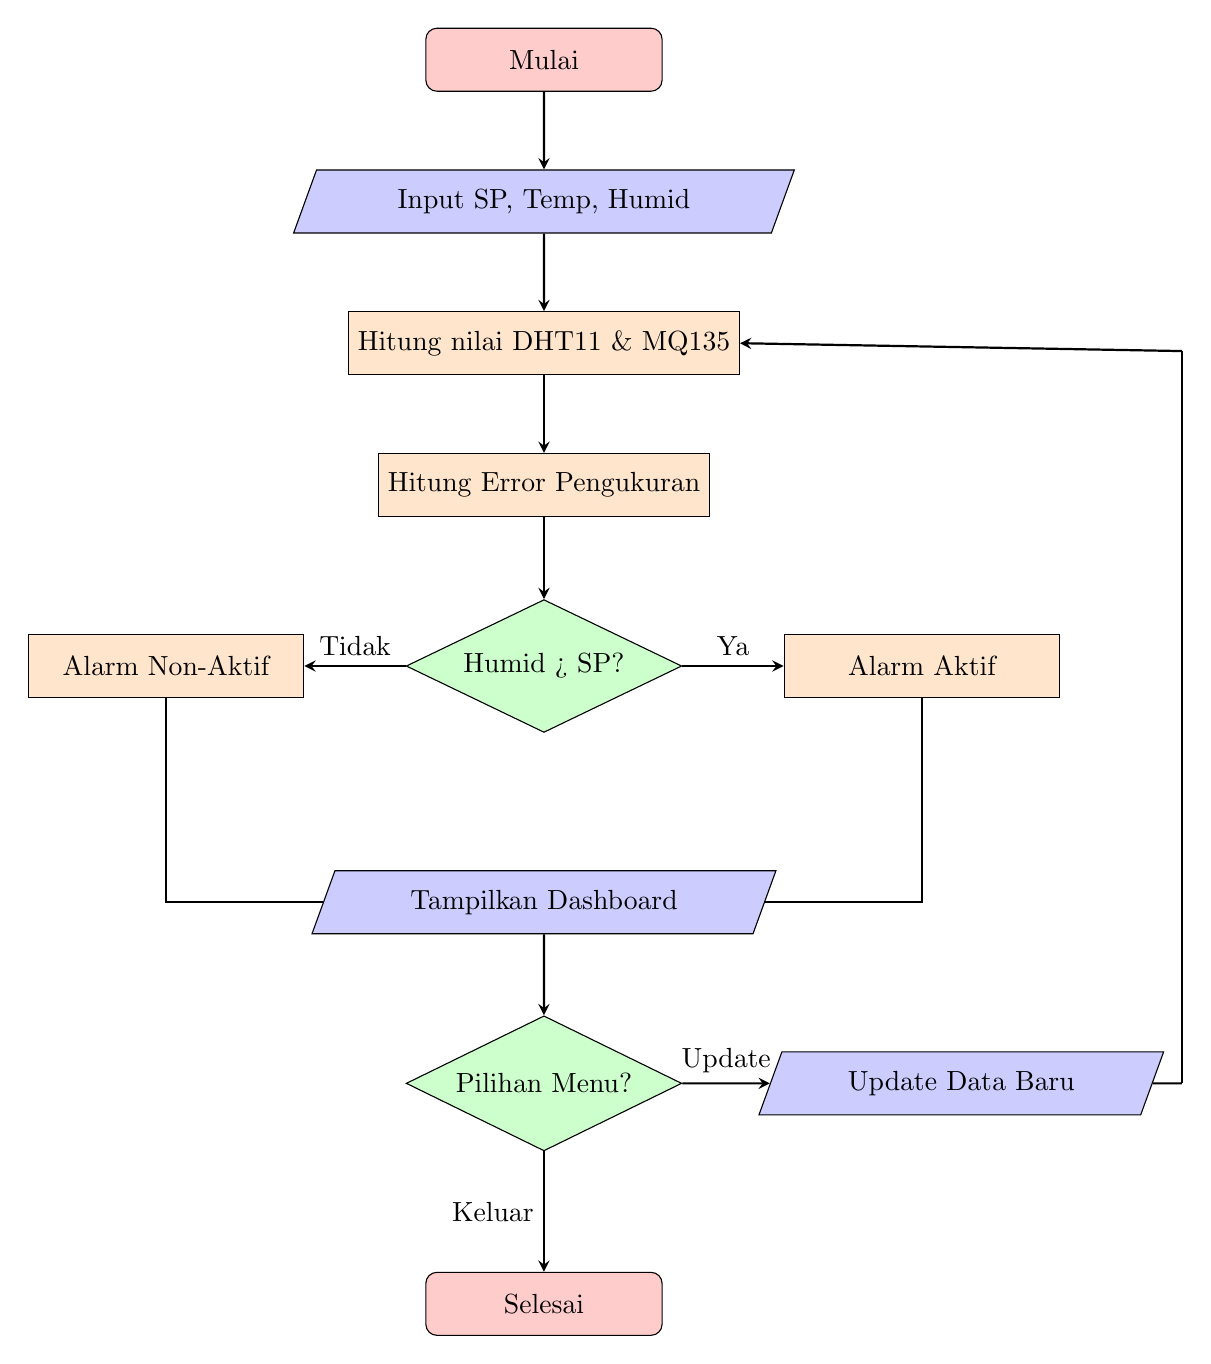
\begin{tikzpicture}[
    node distance=1.8cm, 
    auto,
    startstop/.style={rectangle, rounded corners, minimum width=3cm, minimum height=0.8cm, text centered, draw=black, fill=red!20},
    io/.style={trapezium, trapezium left angle=70, trapezium right angle=110, minimum width=3cm, minimum height=0.8cm, text centered, draw=black, fill=blue!20},
    process/.style={rectangle, minimum width=3.5cm, minimum height=0.8cm, text centered, draw=black, fill=orange!20},
    decision/.style={diamond, aspect=2, minimum width=3.5cm, minimum height=1cm, text centered, draw=black, fill=green!20},
    arrow/.style={thick,->,>=stealth}
]

    \node (start) [startstop] {Mulai};
    \node (input) [io, below of=start] {Input SP, Temp, Humid};
    \node (calc1) [process, below of=input] {Hitung nilai DHT11 \& MQ135};
    \node (calc2) [process, below of=calc1] {Hitung Error Pengukuran};
    \node (dec1) [decision, below of=calc2, yshift=-0.5cm] {Humid > SP?};
    \node (alarm_on) [process, right of=dec1, xshift=3cm] {Alarm Aktif};
    \node (alarm_off) [process, left of=dec1, xshift=-3cm] {Alarm Non-Aktif};
    \node (display) [io, below of=dec1, yshift=-1.2cm] {Tampilkan Dashboard};
    \node (menu) [decision, below of=display, yshift=-0.5cm] {Pilihan Menu?};
    \node (stop) [startstop, below of=menu, yshift=-1cm] {Selesai};
    \node (update) [io, right of=menu, xshift=3.5cm] {Update Data Baru};

    \draw [arrow] (start) -- (input);
    \draw [arrow] (input) -- (calc1);
    \draw [arrow] (calc1) -- (calc2);
    \draw [arrow] (calc2) -- (dec1);
    \draw [arrow] (dec1) -- node[anchor=south] {Ya} (alarm_on);
    \draw [arrow] (dec1) -- node[anchor=south] {Tidak} (alarm_off);
    \draw [thick] (alarm_on) |- (display.east);
    \draw [thick] (alarm_off) |- (display.west);
    \draw [arrow] (display) -- (menu);
    \draw [arrow] (menu) -- node[anchor=east] {Keluar} (stop);
    
    \draw [arrow] (menu) -- node[anchor=south] {Update} (update);
    \coordinate [right of=update, xshift=1cm] (p1);
    \coordinate [above of=p1, yshift=7.5cm] (p2);
    \draw [thick] (update) -- (p1);
    \draw [thick] (p1) -- (p2);
    \draw [arrow] (p2) -- (calc1.east);

\end{tikzpicture}
\end{center}

% ==================== 5. PENJELASAN PROGRAM RUST ==================== %
\newpage
\section{Penjelasan Program Rust}
Program menggunakan \textit{library} I/O standar Rust (\texttt{std::io}). Fungsi modular \texttt{input\_angka} menjamin validitas data melalui \textit{error handling} menggunakan \texttt{match} atau \texttt{if let} pada hasil \textit{parsing} string ke float. Struktur program menggunakan \texttt{loop} tak terbatas yang hanya bisa dihentikan jika pengguna memilih menu keluar (\texttt{break}).

% ==================== 6. KONSEP OOP ==================== %
\section{Konsep Pemrograman Berbasis Objek (OOP)}
Pemrograman berbasis objek pada aplikasi ini diimplementasikan melalui enkapsulasi data dalam \texttt{struct Ruangan}. Logika sensor dan kontroler dipisahkan dalam blok \texttt{impl Ruangan}, yang memungkinkan penggunaan metode instansi (\texttt{\&self}) untuk mengakses atribut objek secara aman.

% ==================== 7. IMPLEMENTASI KOMPUTASI NUMERIK ==================== %
\section{Implementasi Komputasi Numerik}
Sistem menerapkan metode numerik sederhana untuk analisis ketidakpastian instrumentasi melalui perhitungan galat (\textit{error}) absolut:
\begin{equation}
    Error = Nilai_{Terbaca} - Nilai_{Aktual}
\end{equation}
Hal ini diterapkan pada fungsi \texttt{error\_temp()} dan \texttt{error\_humid()} guna memantau akurasi sensor virtual terhadap kondisi \textit{ground truth}.
% ==================== 8. HASIL PENGUJIAN ==================== %
\section{Hasil Pengujian}

Pengujian sistem dilakukan dengan menjalankan program simulasi kontrol berbasis teks dan memantau antarmuka \textit{dashboard} pada terminal. Berikut adalah \textit{source code} bahasa Rust yang digunakan sebagai pengendali utama dalam sistem instrumentasi ini:

\begin{lstlisting}
use std::io;

// ============================================================
//  Struct Ruangan — hanya 3 field input utama
// ============================================================
struct Ruangan {
    set_point_lembab: f32,
    temp_aktual: f32,
    humid_aktual: f32,
}

// ============================================================
//  Implementasi Method
// ============================================================
impl Ruangan {
    // Inisialisasi dengan 3 input
    fn new(set_point_lembab: f32, temp_aktual: f32, humid_aktual: f32) -> Ruangan {
        Ruangan {
            set_point_lembab,
            temp_aktual,
            humid_aktual,
        }
    }

    // DHT11: pembacaan sensor = aktual + offset kecil (1 atau 2)
    fn dht11_temp(&self) -> f32 {
        self.temp_aktual + 1.0
    }

    fn dht11_humid(&self) -> f32 {
        self.humid_aktual + 2.0
    }

    // MQ135: CO2 dan NH3 dihitung dari pembacaan humidity DHT11
    fn mq135_co2(&self) -> f32 {
        self.dht11_humid() * 5.0
    }

    fn mq135_nh3(&self) -> f32 {
        self.dht11_humid() * 10.0
    }

    // Cek apakah aktuator alarm harus aktif
    fn aktuator_aktif(&self) -> bool {
        self.humid_aktual > self.set_point_lembab ||
        self.dht11_humid() > self.set_point_lembab
    }

    // Error = pembacaan sensor - aktual
    fn error_temp(&self) -> f32 {
        self.dht11_temp() - self.temp_aktual
    }

    fn error_humid(&self) -> f32 {
        self.dht11_humid() - self.humid_aktual
    }

    // Tampilkan seluruh output
    fn tampilkan(&self) {
        let status_alarm = if self.aktuator_aktif() { "Aktif" } else { "Non-Aktif" };
        println!("\n========================================");
        println!("       DASHBOARD MONITORING RUANGAN     ");
        println!("========================================");
        
        // --- DHT11 ---
        println!("\n[ Pembacaan Sensor DHT11 ]");
        println!("  Temperature : {:.1} °C", self.dht11_temp());
        println!("  Humidity    : {:.1} %", self.dht11_humid());
        
        // --- MQ135 ---
        println!("\n[ Pembacaan Sensor MQ135 ]");
        println!("  CO2 : {:.1} ppm", self.mq135_co2());
        println!("  NH3 : {:.1} ppm", self.mq135_nh3());
        
        // --- Controller ESP32 ---
        println!("\n[ Controller ESP32 ]");
        println!("  Sensor (DHT11 dan MQ135) : Aktif");
        println!("  Aktuator (Alarm)         : {}", status_alarm);
        
        // --- Alarm ---
        println!("\n[ Alarm ]");
        if self.aktuator_aktif() {
            println!("  Status : AKTIF  !! Humidity melebihi Set Point !!");
        } else {
            println!("  Status : Non-Aktif");
        }

        // --- Error ---
        println!("\n[ Error Sensor ]");
        println!("  Error Temperature : {:.1} °C", self.error_temp());
        println!("  Error Humidity    : {:.1} %", self.error_humid());

        println!("\n========================================\n");
    }
}

// ============================================================
//  Helper input
// ============================================================
fn input_angka(pesan: &str) -> f32 {
    loop {
        println!("{}", pesan);
        let mut input = String::new();
        io::stdin().read_line(&mut input).unwrap();
        if let Ok(angka) = input.trim().parse() {
            return angka;
        } else {
            println!("Input salah! Masukkan angka.");
        }
    }
}

// ============================================================
//  Main
// ============================================================
fn main() {
    println!("========================================");
    println!("    SISTEM MONITORING SENSOR v3.0       ");
    println!("========================================");
    let sp_lembab    = input_angka("\nMasukkan Set Point Humidity (%): ");
    let temp_aktual  = input_angka("Masukkan Temperature Aktual (°C): ");
    let humid_aktual = input_angka("Masukkan Humidity Aktual (%): ");
    
    let mut ruangan = Ruangan::new(sp_lembab, temp_aktual, humid_aktual);
    ruangan.tampilkan();

    // Loop menu update
    loop {
        println!("MENU: [1] Update Nilai  [2] Keluar");
        let pilihan = input_angka("Pilih (1/2): ");

        if pilihan == 1.0 {
            let t = input_angka("\nTemperature Aktual baru (°C): ");
            let h = input_angka("Humidity Aktual baru (%): ");
            ruangan.temp_aktual  = t;
            ruangan.humid_aktual = h;
            ruangan.tampilkan();
        } else if pilihan == 2.0 {
            println!("Sistem Dimatikan.");
            break;
        } else {
            println!("Pilihan tidak valid.");
        }
    }
}
\end{lstlisting}

Berdasarkan implementasi kode di atas, pengujian dilakukan dalam dua skenario dinamis untuk melihat respons logika kontrol aktuator terhadap perubahan nilai sensor di lingkungan virtual.

\subsection{Skenario 1: Kondisi Lingkungan Normal (Alarm Non-Aktif)}

Pada pengujian pertama, sistem membaca data dari sensor dengan hasil suhu lingkungan $51.0^\circ \text{C}$ dan kelembaban $42.0\%$. Karena nilai kelembaban terbaca masih berada di bawah atau setara dengan batas \textit{Set Point} yang ditetapkan oleh operator, metode \texttt{aktuator\_aktif()} bernilai \textit{false}. Oleh karena itu, Controller ESP32 menahan aktuator dalam status \textbf{Non-Aktif}. 

Sistem juga menunjukkan akurasi kalkulasi error sensor secara presisi menggunakan operasi numerik standar (\texttt{f32}), yang menghasilkan nilai galat konstan sebesar $1.0^\circ \text{C}$ untuk suhu dan $2.0\%$ untuk kelembaban sesuai dengan asumsi \textit{offset} pada sensor DHT11 virtual. Ekstrapolasi gas pada MQ135 juga berjalan baik dengan kalkulasi $CO_2$ sebesar $210.0$ ppm dan $NH_3$ sebesar $420.0$ ppm.
\newpage
\subsection{Skenario 2: Peringatan Ambang Batas (Alarm Aktif)}

Pada pengujian kedua, fitur \textit{Update Nilai} digunakan untuk memasukkan data aktual baru (suhu $2.0^\circ \text{C}$ dan kelembaban $3.0\%$). Pada skenario ini, diasumsikan batas \textit{Set Point} yang diatur sangat ketat (misalnya di bawah $3.0\%$). Seperti terlihat pada Gambar \ref{fig:kondisi_bahaya}, ketika variabel \texttt{self.dht11\_humid()} melampaui \textit{Set Point}, kontrol sistem langsung dieksekusi secara \textit{real-time}. 

Peralihan Boolean menjadi \textit{true} seketika memerintahkan aktuator untuk mengubah status menjadi \textbf{AKTIF}, ditandai dengan interupsi pesan peringatan ``!! Humidity melebihi Set Point !!''. Pembacaan MQ135 turut menurun secara proporsional menjadi $CO_2$ sebesar $15.0$ ppm dan $NH_3$ sebesar $30.0$ ppm. Hal ini membuktikan bahwa enkapsulasi dan aliran logika program Rust yang dikembangkan telah responsif untuk diterapkan pada \textit{plant} instrumentasi.
% ==================== 9. ANALISIS HASIL ==================== %
\section{Analisis Hasil}
Analisis menunjukkan bahwa sistem responsif terhadap perubahan data dinamis. Penggunaan tipe data \texttt{f32} memberikan presisi yang cukup untuk angka di belakang koma pada pembacaan suhu dan kadar gas ppm. Integrasi logika kontrol pada metode \texttt{aktuator\_aktif()} berhasil menyatukan kondisi sensor digital dan kondisi aktual sesuai standar sistem IoT.
% ==================== 10. KESIMPULAN ==================== %

\section{Kesimpulan}
Aplikasi monitoring berbasis Rust ini berhasil memenuhi kriteria ETS, mencakup penggunaan OOP, validasi input, dan komputasi numerik. Sistem simulasi ini membuktikan bahwa Rust sangat efektif digunakan untuk logika kontrol instrumentasi cerdas.
% ==================== DAFTAR PUSTAKA ==================== %
\begin{thebibliography}{99}

\bibitem{garg2025}
R. Garg, A. Kumar, R. Dayana, and S. Singh, "Advanced Air Quality Monitoring System using IoT and Sensor Technology," \textit{2025 3rd International Conference on Intelligent Data Communication Technologies and Internet of Things (IDCIoT)}, Chennai, India, 2025, pp. 687-692.

\bibitem{chanthakit2018}
S. Chanthakit and C. Rattanapoka, "MQTT Based Air Quality Monitoring System using NodeMCU and Node-RED," \textit{2018 Seventh ICT International Student Project Conference (ICT-ISPC)}, Bangkok, Thailand, 2018, pp. 1-5.

\end{thebibliography}

\end{document}